\documentclass{article}
\usepackage{amsmath}
\usepackage{amssymb}
\usepackage{graphicx}
\usepackage{xcolor}
\usepackage{hyperref}

\hypersetup{urlcolor=cyan}

\title{OT intro}
\author{Qi Wang}
\date{\today}

\begin{document}

\maketitle

\begin{abstract}
   Reference literatures: Cambridge note for OT, computational OT from Gabriel Peyre, Benamou-Brenier formulation, etc. For packages of OT solvers, refering to \href{https://github.com/PythonOT/POT}{POT} for a Python binding of Sinkhorn and Gromov-Wasserstein solvers.
\end{abstract}

\section{Optimal transport}
\subsection{Monge's problem}
The very beginning of the OT problem: Monge's problem. Monge's problem describes the existence of a map $T$ that transports one distribution $P$ to another $Q$ with the minimum cost $c^*$. Here $P,Q \in \mathcal{P}(X), \mathcal{P}(Y)$ respectively, and  both $X,Y \in \mathbb{R}^{d}$. The original cost function in Monge problem is $L_{1}$ cost, which is significantly harder than $L_{2}$ cost.

\begin{equation}
    \inf_{T} \int_{x\in \mathbb{R}^{d}} c(x, T(x)) dP(x)
\end{equation}
where $T: X \rightarrow Y$ subject to $T_{\#}P = Q$. 


\subsection{Kantorovich's problem}
With the Monge's problem being too ill-posed, Kantorovich relaxed the problem to the OT problem where each element in the source distribution is separable and each one in target distribution can be composed from multiple sources. Minimising the Kantorovich formulation is to find the optimal transport plan $\pi \in \mathcal{P}(X \times Y)$ that minimizes the cost $c$.

\begin{equation}
    \inf_{\pi} \int_{X \times Y} c(x,y) d\pi(x,y)
\end{equation}
where $\pi(x,y) \in \Pi(P, Q)$, and $\pi(x,y) = \{\Pi \in \mathbb{R}^{n\times m}_{+} | \Pi1_{m} = P, \Pi^{T}1_{n} = Q\}$ denotes the marginals can be acquired from the coupling.

\subsection{Dynamic process of transportation}
Considering the transportation process as a dynamic process, to not confuse the notation with discrete OT, we can define the transportation plan $p_{t}(x) = p(t,x)$ as a dynamic process that transports the mass from $p_{0}(x) = P$ to $p_{1}(x) = Q$ and velocity field $v(t,x)$.

\textcolor{red}{add the derivation of the continuity equation from fokker-planck equation}

From the continuity equation, we have the following equation:
\begin{equation}
    \frac{\partial{p_{t}}}{\partial{t}} + \nabla \cdot (p_{t}v_{t}) = 0
\end{equation}

meanwhile, the kinetic energy of the transportation process is defined as:

\begin{equation}
    \int_{0}^{1} \int_{X} \frac{1}{2} \lVert v_{t}(x) \rVert^{2} p_{t}(x) dx dt
\end{equation}

From \textbf{Benamou-Brenier formulation}, we know the OT map $T$ is the gradient of a convex function $\phi$, \emph{i.e.} $T = \nabla \phi$, which pushes forward the initial distribution $P$ to the target distribution $Q$. 

\subsection{Entropic regularization for OT}
The idea of entropic regularization is to add a entropy term to the original OT problem, which makes the problem more well-posed and easier to solve.

\begin{equation}
    \inf_{\pi} \int_{X \times Y} c(x,y) d\pi(x,y) + \lambda H(\pi)
\end{equation}

where $H(\cdot)$ denotes the Shannon entropy of the transportation plan $\pi$: $H(\pi) = -\int_{X \times Y} \pi \log(\pi) d\pi$ (for the sake of simplicity, abused notation: $\pi = \pi(x,y)$). As can be seen, the entropy $H(\cdot)$ increases when the distribution is more uniform(homogenous), vice versa. Such entropic regularised OT distance is also called \textbf{Sinkhorn distance}.

Thus, one can tell that the entropic regularisation is a smoothing operation on the original OT problem, which enforces the transportation plan to be more homogeneous with a trade-off to loss specificity (exactness) of distribution match. However, from a different point of view, the entropic reguarisation term can be seen similiar as a ridge regularisation, which increase  the generalisation of the model.


From the Fig.\ref{fig:sinkorn_geometry}, we can see the original OT can be solved in linear programming, where the intersection points on $U(r,c)$ are the optimal solution $P^{*}$. However, the entropic regularised OT problem is a smoothed version of the original OT problem, whose optimal points are $P^{*}_{\lambda}$. If $\lambda \rightarrow 0$, then $P^{*}_{\lambda} \rightarrow rc^{T}$, which is a uniform distribution; else if $\lambda \rightarrow \infty$, then $P^{*}_{\lambda} \rightarrow P^{*}$, which is the original OT solution.

\textbf{Appliations of entropic regularisation}: 
\begin{enumerate}
    \item distribution matching, which minimises the Sinkhorn distribution distance;
    \item distance measure, which is more flexible than using a KL divergence to measure the distance between two distributions, but can enforce prior knowledges;
\end{enumerate}

\begin{figure}[h]
    \centering
    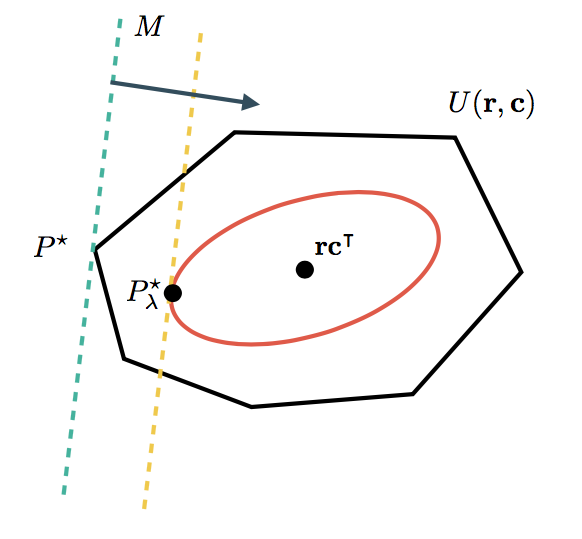
\includegraphics[width=0.8\textwidth]{./figs/geometry.png}
    \caption{Geometrical illustration of the OT metric landscape and its entropic regularized one (\emph{red}). Note the optimisation landscape is smoothed for entropic regularisation loss}
    \label{fig:sinkorn_geometry}
\end{figure}

\subsection{Unbalanced OT}
\subsection{Low-rank OT}

\section{Main Content}
This is the main content section.

\section{Conclusion}
This is the conclusion section.

\end{document}